\section{MOS Transistoren}

\subsection{Dotierung}
\begin{center}
    \begin{tabular}{lll}
        \textbf{Dotierung:}          & N-dotiert            & P-dotiert \\
        \textbf{Unreinheit:}         & Aluminium (HG III)   & Phosphor / Arsen (HG V) \\
        \textbf{Majoritätsträger:}   & Elektronen           & Löcher \\
        \textbf{Minoritätsträger:}   & Löcher               & Elektronen \\
    \end{tabular}
\end{center}


\subsection{MOS-Kapazität}
\begin{minipage}[t]{0.5\columnwidth}
    Minoritätsträger werden an das Gate gezogen.
    Die entstandene Raumladungszone weist bei ausreichend hoher Gate-Spannung einen Minoritätsträgerüberschuss auf, ist also in der Funktion \textbf{komplementär} zum Substrat dotiert.
\end{minipage}
\hfill
\begin{minipage}[t]{0.48\columnwidth}
    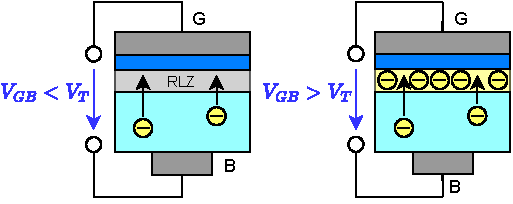
\includegraphics[width=\columnwidth, align=t]{images/02_MOS_kapazitaet.pdf}
\end{minipage}


\subsection{MOS-Transistoren}
Werden links und rechts vom MOS-Kondensator komplementär zum Substrat dotierte Regionen (Drain und Source) erstellt, so kann ohne Gatespannung aufgrund der PN-Übergänge kein Strom vom Drain zur Source (oder umgekehrt) fliessen.
Wird nun eine Spannung am Gate angelegt, so entsteht die Minoritätsträger-Leitende Raumladungszone - der Kanal.
Dieser verbindet Drain und Source, es kann also ein Strom fliessen.

\vspace{-0.2cm}

\begin{center}
    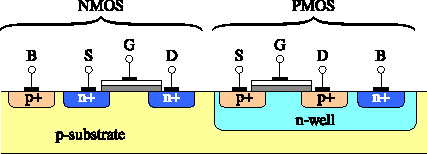
\includegraphics[width=0.5\columnwidth, align=t]{images/02_CMOS.pdf}
\end{center}


\subsubsection{Übersicht und Symbole}

\begin{minipage}[t]{0.48\columnwidth}
    Durch Vordotierung des Kanals kann der Transistor ohne Gate-Spannung leitend gemacht werden (Verarmungstyp, selbstleitend).
    Eine negative Gate-Spannung kann den Kanal dann abschnüren. \\
    \rightarrow\ hier nicht weiter behandelt

    \smallskip

    \textbf{Der Bulk wird nur eingezeichnet, wenn dieser \myul{nicht} mit $\bm{V_{\rm DD}}$ bzw. $\bm{V_{\rm SS}}$ verbunden ist.}
    Deshalb werden meist die vereinfachten Symbole verwendet:

    \vspace{-0.3cm}

    \begin{center}
        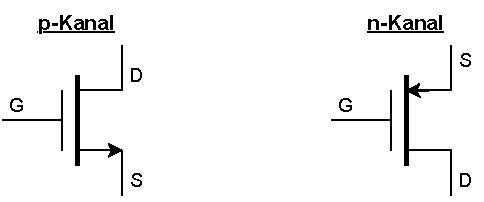
\includegraphics[width=0.8\columnwidth, align=t]{images/02_MOSFET_symbole_vereinfacht.pdf}
    \end{center}
\end{minipage}
\hfill
\begin{minipage}[t]{0.5\columnwidth}
    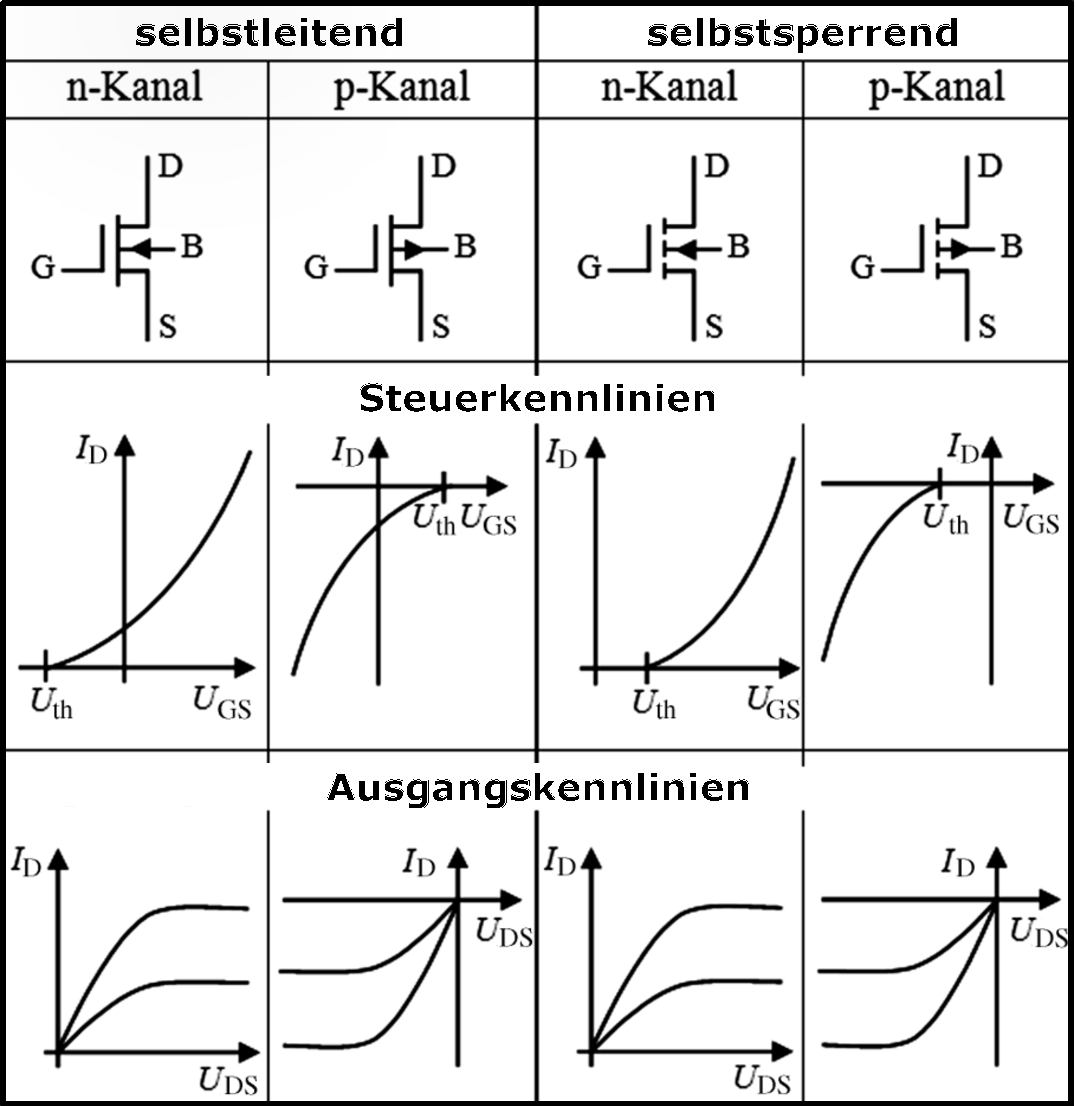
\includegraphics[width=\columnwidth, align=t]{images/02_MOSFET_uebersicht.pdf}
\end{minipage}



\subsubsection{Modelle}
In Cadence sind verschiedene Modelle hinterlegt:

\textbf{Spice Modell 11:} Das Modell 11 beinhaltet ca. 100 Parameter und ist entsprechend genau.

\textbf{Spice Modell 1:} Vergleichbar mit dem Handrechenmodell, welches zwar weniger genau, dafür aber viel einfacher ist. Dennoch beinhaltet es bereits 40 Parameter.

\subsection{Ausgangskennlinie -- Arbeitsbereiche}
 
Die Ausgangskennlinie beschreibt den Zusammenhang $I_D = f(V_{DS}) \big|_{V_{GS} = \text{konst}}$

\begin{minipage}[t]{0.5\columnwidth}
    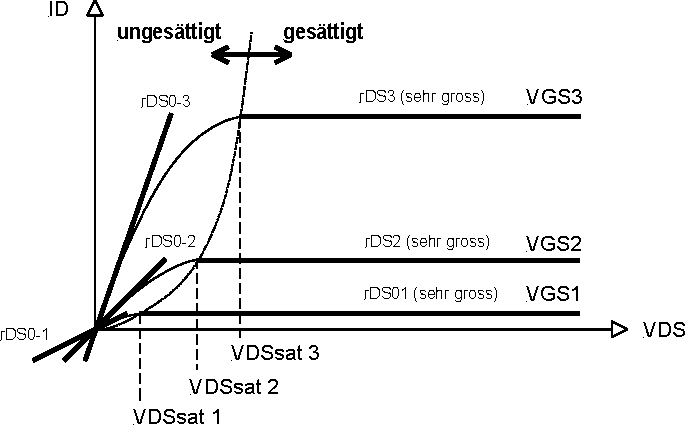
\includegraphics[width=\columnwidth, align=t]{images/02_MOSFET_ausgangskennlinien.pdf}
\end{minipage}
\hfill
\begin{minipage}[t]{0.48\columnwidth}
    Zwei Arbeitsbereiche: 

    \begin{outline}
        \1 ungesättig (gesteuerter Widerstand)
        \1 gesättigt (Stromquelle)
    \end{outline}

    \medskip

    Die Sättigungsgrenze $V_{\rm DS, sat}$ ist abhängig vom \textbf{Kanalzustand}:

    \begin{outline}
        \1 \textbf{weak inversion:} \\
            $V_{\rm DS, sat} = V_{\rm eff} \approx 5 \cdot V_{\rm temp} \approx \qty{130}{\milli \volt}$ 
        \1 \textbf{strong inversion:} \\
            $V_{\rm DS, sat} = V_{\rm eff} = V_{GS} - V_T$ 
    \end{outline}
\end{minipage}



\subsection{Transferkennlinie -- Ausgangsstrombereiche}


\begin{minipage}[t]{0.55\columnwidth}
    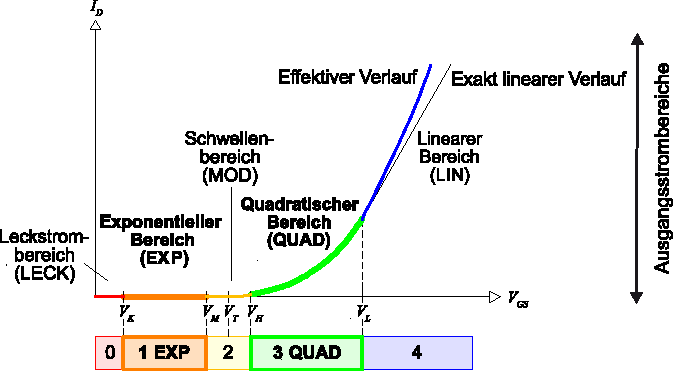
\includegraphics[width=\columnwidth, align=t]{images/02_MOSFET_transferkennlinie.pdf}
\end{minipage}
\hfill
\begin{minipage}[t]{0.42\columnwidth}
    Die Transferkennlinie beschreibt den Zusammenhang $I_D = f(V_{GS})$ 

    \smallskip

    Dabei werden \textbf{5 Ausgangsstombereiche} unterschieden. Diese hängen mit dem \textbf{Kanalzustand} zusammen.

    \smallskip

    Des Weiteren gibt es die Bereiche:

    \begin{outline}
        \1 Sub Threshold: $V_{GS} < V_T$
        \1 Above Threshold: $V_{GS} > V_T$
    \end{outline}
\end{minipage}


\para{Ausgangsstrombereiche}

\scalebox{0.8}{
\begin{tabular}{|l|l|l|}
    \hline
    \textbf{Bereich}                    & \textbf{Mathem. Charakterisierung}            & \textbf{Zugrundeliegender phys. Effekt}                       \\  
    \hline
    \rowcolor[HTML]{F4CCCC} 
    LECK                                & $I_D$ erreicht Minimalwert, der nicht         & Drain- und Source-Substratdiode haben                         \\
    \rowcolor[HTML]{F4CCCC} 
                                        & weiter unterschritten werden kann             & Leckströme ins Subsstrat                                      \\
    \hline
    \rowcolor[HTML]{FFE5BB} 
    EXP                                 & $I_D$ steigt exponentiell mit $V_{GS}$        & Kanal zeigt \textbf{weak inversion}                           \\
    \hline
    \rowcolor[HTML]{FFF2CC} 
    MOD                                 & Keine 'handliche' Formel für $I_D$            & Kanal zeigt \textbf{moderate inversion}                       \\
    \hline
    \rowcolor[HTML]{D9EAD3} 
    QUAD                                & $I_D$ steigt quadratisch mit $V_{GS}$         & Kanal zeigt \textbf{strong inversion}                         \\
    \hline
    \rowcolor[HTML]{CFE2F3} 
    LIN                                 & $I_D$ steigt annähernd linear mit $V_{GS}$    & Geschwindigkeitssättigung der Ladungsträger im Kanal          \\
    \rowcolor[HTML]{CFE2F3} 
                                        & (halb QUAD, halb LIN)                         & im Kanal (nicht weiter beschleunigbar)                        \\
    \hline
\end{tabular}
}

\smallskip

\textbf{Hinweis:} Die Inversion des Kanals beschreibt, wie sehr sich die Polarität geändert ('invertiert') hat. 
Bei einem n-Kanal FET ist der Kanal ursprünglich p-leidend.
Wird der Kanal invertiert, so wird er (schwach, moderat oder start) n-leitend. 


\subsection{Ersatzschaltungen}

Je nach Arbeitsbereich (gesättigt / ungesättigt) müssen verschiedene Ersatzschaltungen verwendet werden.

\begin{minipage}[t]{0.48\columnwidth}
    \raggedright

    \subsubsection*{Ungesättigt}

    Gesteuerter Widerstand \rightarrow\ $I_D = f(V_{DS})$
    
    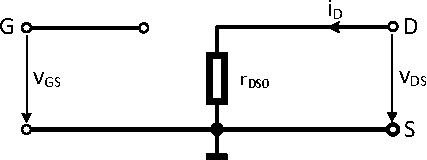
\includegraphics[width=\columnwidth, align=t]{images/02_MOSFET_ersatzschaltung_ungesaettigt.pdf}

    \smallskip
    Je kleiner $r_{\rm DS0}$, desto steiler die Geraden links im Ausgangskennlinienfeld

\end{minipage}
\hfill
\begin{minipage}[t]{0.48\columnwidth}
    \raggedright

    \subsubsection*{Gesättigt}

    Stromquelle \rightarrow\ $I_D = f(V_{GS})$

    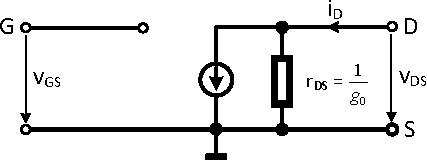
\includegraphics[width=\columnwidth, align=t]{images/02_MOSFET_ersatzschaltung_gesaettigt.pdf}

    \smallskip
    Je grösser $r_{\rm DS}$, desto flacher die Geraden rechts im Ausgangskennlinienfeld
\end{minipage}


\subsection{Berechnung des Drainstroms}

Die Berechnung des Drainstroms hängt sowohl von Arbeitsbereich (gesättigt / ungesättig), als auch vom Ausgangsstrombereich (bzw. der Kanaliversion) ab!


\subsubsection{Strong Inversion}

\vspace{-0.3cm}

% $$ \boxed{ \text{QUAD-Bereich: } V_H(I_D) < V_{GS} < V_L(I_D) } \qquad \qquad \beta = \mu \cdot C_{\text{OX}} \cdot \frac{W}{L} $$
$$ \boxed{ \text{QUAD-Bereich:} \quad V_H(I_D) \leq V_{GS} < V_L(I_D) \quad \text{bzw.} \quad I_H \leq I_D < I_L } $$  %NOTE: Bedingung für Ströme aus Ü3, 3.6.4 1)

\resizebox{\columnwidth}{!}
{
    \renewcommand{\arraystretch}{1.5}
    \begin{tabular}{@{}l c | c@{}}
                & \textbf{Ungesättigt:} \quad $\bm{| V_{DS} | < | V_{GS} - V_T |}$                                                              & \textbf{Gesättigt:} \quad $\bm{| V_{DS} | \geq | V_{GS} - V_T |}$                         \\
        NMOS:   & $I_D = \beta \cdot \bigg[ (V_{GS} - V_T) V_{DS} - \frac{V_{DS}^2}{2} \bigg] \cbl{\cdot (1 + \lambda \cdot \Delta V_{DS})}$    & $I_D = \frac{\beta}{2} (V_{GS} - V_T)^2 \cbl{\cdot (1 + \lambda \cdot \Delta V_{DS})}$    \\
        \midrule
        PMOS:   & $I_D = - \beta \cdot \bigg[ (V_{GS} - V_T) V_{DS} - \frac{V_{DS}^2}{2} \bigg] \cbl{\cdot (1 - \lambda \cdot \Delta V_{DS})}$  & $I_{D} = - \frac{\beta}{2} (V_{GS} - V_T)^2 \cbl{\cdot (1 - \lambda \cdot \Delta V_{DS})}$
    \end{tabular}
    \renewcommand{\arraystretch}{1}
}

\medskip

\textbf{Ohne} Berücksichtigung der \textbf{Kanallängenmodulation:} \cbl{blauen Term $=1$} bzw $\lambda = 0$ setzen



% NOTE [Simi] @Flurin: Hier noch dein Vorschlag der Darstellung (mit NMOS / PMOS Ergänzung):
% Jetzt können wir streiten, welchen wir nehmen wollen :P

% \resizebox{\columnwidth}{!}
% {
%     \renewcommand{\arraystretch}{1.5}
%     \begin{tabular}{l c|c}
%                 & \textbf{Ungesättigt:} \quad $\bm{| V_{\rm DS} | < | V_{GS} - V_T |}$                          & \textbf{Gesättigt:} \quad $\bm{| V_{\rm DS} | \geq | V_{GS} - V_T |}$             \\
%         NMOS:   & $I_{\rm D, ideal} = \beta \cdot \bigg[ (V_{GS} - V_T) V_{DS} - \frac{V_{DS}^2}{2} \bigg]$     & $I_{\rm D, ideal} = \frac{\beta}{2} (V_{GS} - V_T)^2 $                            \\
%         NMOS:   & $I_{\rm D, real} = I_{\rm D, ideal} \cdot (1 + \lambda \cdot \Delta V_{DS})$                  & $I_{\rm D, real} = I_{\rm D, ideal} \cdot (1 + \lambda \cdot \Delta V_{DS})$      \\
%         \midrule
%         PMOS:   & $I_{\rm D, ideal} = - \beta \cdot \bigg[ (V_{GS} - V_T) V_{DS} - \frac{V_{DS}^2}{2} \bigg]$   & $I_{\rm D, ideal} = - \frac{\beta}{2} (V_{GS} - V_T)^2$                           \\
%         PMOS:   & $I_{\rm D, real} = I_{\rm D, ideal} \cdot (1 - \lambda \cdot \Delta V_{DS})$                  & $I_{\rm D, real} = I_{\rm D, ideal} \cdot (1 - \lambda \cdot \Delta V_{DS})$      
%     \end{tabular}
%     \renewcommand{\arraystretch}{1}
% }



\paragraph{Transkonduktanz-Parameter $\bm{\beta}$}

\begin{minipage}[c]{0.78\columnwidth}
    $\beta$ ist abhängig davon, ob der Transistor gesättigt ist. 
    In der Praxis wird diese Unterscheidung jedoch \textbf{nicht} gemacht. 
    Im \textbf{Design} kann $\beta$ durch das Verhältnis von Kanalbreite $W$ und -länge $L$ beeinflusst werden.
\end{minipage}
\hfill
\begin{minipage}[c]{0.2\columnwidth}
    $$ \beta = \underbrace{ \mu C_{\rm OX} }_{\beta_0} \frac{W}{L} $$
\end{minipage}


%TODO: [Flurin] NMOSI und PMOSI V2S12
% NOTE: [Simi] @ Flurin: Bist du sicher, dass du diese Slide meinst...? 



%TODO: [Flurin] V3S9 nochmal studieren, macht iwie noch nicht so sinn.
\paragraph{Kanallängenmodulation $\bm{\lambda$} und Early-Spannung $\bm{V_E}$}

\begin{minipage}[c]{0.7\columnwidth}
    % Die Early-Spannung $V_E = a_E \cdot L$ setzt sich zusammen aus dem technologieabhängigen Early-Faktor $a_E$ und der Kanallänge $L$.
    Die Kanallängenmodulation beschreibt die Nichtidealität der spannungsgesteurten Stromquelle (im Sättigungsbetrieb). \\
    Idealfall: $\lambda = 0$ \rightarrow\ $L = \infty$
\end{minipage}
\hfill
\begin{minipage}[c]{0.28\columnwidth}
    $$ \lambda = \frac{1}{V_E} = \frac{1}{a_E \cdot L} $$
    % \overset{V_E >> V_{DS}}{\approx} \frac{1}{V_E}
\end{minipage}

\smallskip

\textbf{Achtung:} $\bm{V_E}$ ist typischerweise negativ, wird jedoch \textbf{immer positiv angegeben}. 
Grafisch entspricht $V_E$ der Spannung $V_{DS}$, bei welcher die Verlängerung der Ausgangskennlinie (Sättigung) die $V_{DS}$-Achse schneidet.


%CHECK: Ich finde die Herleitung aus V3S9 überflüssig. Evtl. macht die Grafik zur Early-Spannung sinn? Braucht halt viel platz...
% [Simi] @Flurin: Ja, auf die Herleitung würde ich auch verzichten. Das Bild wäre allenfalls sinnvoll. 
% Aus Platzgründen habe ich etws 'Prosa' zur Early-Spannung geschrieben... Wirklich toll ist der Text aber auch nicht...


\paragraph{Body-Effekt}
Der Body-Effekt beschreibt die \textbf{Abhängigkeit der Schwellenspannung} $\bm{V_T}$ von der Source-Bulk-Spannung $V_{SB}$ als
$$ V_T = V_{T0} \pm \Delta V_T \quad \text{mit} \quad \Delta V_T = \gamma\left(\sqrt{\abs{V_{SB}} + \abs{2\Phi_F}}-\sqrt{\abs{2\Phi_F}}\right)$$

\rightarrow\ Body-Effekt nur wirksam, wenn $V_{SB} \neq \qty{0}{\volt}$ \\
\rightarrow\ Reminder: Bulk nur gezeichnet, wenn nicht auf $V_{DD}$ oder $V_{SS}$

\medskip
% --------------------------------------------------------------------------------------------------------------------

Das Fermi-Potential
\[
    \Phi_F = kT/q \ln(N_A/n_i)
\]
mit 
\begin{tabular}{rl}
    $n_i$:& Intrinsische ladungsdichte von Silizium\\
    $N_A$:& Ladungsdichte der Akzeptoren
\end{tabular}
ist Prozess- wie auch Temperaturabhängig.
Zudem ist er abhängig der Dotierungsstärke.



Body-Effekt-Konstante
\[
    \gamma \overset{\approx}{n-Dotierung} \qty{1.46}{\sqrt{\volt}}
\]
\[
    \gamma \overset{\approx}{p-Dotierung} \qty{1.08}{\sqrt{\volt}}
\]



\subsubsection{Weak Inversion}

\vspace{-0.3cm}

% $$ \boxed{ \text{EXP-Bereich: } V_K(I_D) < V_{GS} < V_M(I_D) \qquad \qquad V_M(I_D) = V_T(I_D) - x_M(I_D) } $$
$$ \boxed{ \text{EXP-Bereich: } V_K(I_D) < V_{GS} \leq V_M(I_D) \qquad \qquad I_K < I_D \leq I_M } $$  %NOTE: Bedingung für Ströme aus Ü3, 3.6.5 1)


%TODO bzw CHECK [Simi] @Flurin Vtemp Formel auch irgendwo ergänzen? Wert für Vtemp in Übungen immer aus Technologiehandbuch gegeben
% CHECK [Flurin] @Simi Würde ich in die FoSa nemen falls an der Prüfung nicht gegeben. Habe aber noch einen disclaimer eingebaut.
Dabei wird $V_{\rm temp}$ oft vom Technologiehandbuch gegeben. 

Alternativ kann sie als 

\begin{minipage}{0.4\columnwidth}
    \[
        V_{\rm temp} = \frac{kT}{q} \approx \qty{130}{\milli\volt}
    \]
\end{minipage}
\hfill
\begin{minipage}{0.5\columnwidth}
    \begin{tabular}{rl}
        $k$: & Boltzmann-Konstante \\
        $q$: & Elementarladung \\
        $T$: & Temperatur in Kelvin \\
    \end{tabular}
\end{minipage}

% CHECK: Ist das tatsächlich eine approximation? Was stimmt nicht daran?
% CHECK: Wovon kommen die 130 mV? -> Gesehen in Quiz zu Woche 2
approximativ berechnet werden.

\renewcommand{\arraystretch}{1.5}
\begin{ctabular}{c|c}
    \textbf{Ungesättigt}                                                                                                & \textbf{Gesättigt}                                                    \\
    $I_D = I_M \cdot \e^{\frac{V_{GS} - V_M}{n_M \cdot V_\text{temp}}} \cdot (1 - \e^{-\frac{V_{DS}}{V_\text{temp}}})$  & $I_D = I_M \cdot \e^{\frac{V_{GS} - V_M}{n_M \cdot V_\text{temp}}}$
\end{ctabular}
\renewcommand{\arraystretch}{1}

\paragraph{Temparaturspannung}
\[
    V_{temp} = \frac{k T}{q} \approx \qty{86.2}{\micro\volt\per\kelvin} \cdot T
\]

\paragraph{Spezifischer Drainstrom}
\[
    I_M = \frac{W}{L} I_{M, 0}
\]

\paragraph{Subthreshold Slope Factor}
\[
    n_M = 1 + \frac{\gamma}{2\sqrt{V_{SB}+\Phi_0}} \quad \text{mit} \quad \Phi_0 = 2 \Phi_F \approx \qty{0.6}{\volt}
\]

\paragraph{Kanallängenmodulation}
\[
    \lambda = \frac{1}{V_E} \approx \frac{1}{a_E L}
\]

\paragraph{Transkonduktanz-Parameter}
\[
    \beta = \frac{W}{L}\beta_0 = \mu C_{OX}
\]
(unter Vernachlässigung der Abhängigkeit von der Sättigung.)

\subsubsection{Bereiche ohne Berechnungsformeln}

In den drei verbleibenden Bereichen sind \textbf{keine Berechnungsformeln für} $\bm{I_D}$ vorhanden.

\smallskip

\begin{minipage}[c]{0.48\columnwidth}
    \renewcommand{\arraystretch}{1.2}
    \begin{ctabular}{lll}
        \textbf{Bereich}    & \textbf{Grenzen}                  \\
        LECK                & $V_K(I_D) < V_{GS} < V_M(I_D)$    \\ 
        MOD                 & $V_M(I_D) < V_{GS} < V_H(I_D)$    \\ 
                            & $V_H(I_D) = V_T(I_D) + x_H(I_D)$  \\
        LIN                 & $V_L(I_D) < V_{GS}$               \\ 
    \end{ctabular}
\end{minipage}
\hfill
\begin{minipage}[c]{0.48\columnwidth}
    Im MOD-Bereich (moderate inversion) liefern die Formeln der weak bzw. strong inversion katastrophal falsche Resultate!

    \smallskip

    Es ist daher enorm wichtig, den Arbeitsbereich des Transistors korrekt zu bestimmen.
\end{minipage}


\subsection{Modellierung}
\subsubsection{Bestimmung des Arbeitspunkts}
Um den Zustand eines MOS-FET zu bestimmen, wird wie folgt vorgegangen:
\begin{enumerate}
    \item $V_{GS}$ bestimmen
    \item Ausgangsstrombereich (weak, strong inversion, \ldots) anhand von Vergleich von $V_{GS}$ mit $V_K$, $V_M$, $V_T$, $V_H$ und $V_L$
    \item $V_{DS}$ ermitteln
    \item $V_{DS, sat}$ ausrechnen
    \item Ausgangsspannungsbereich durch vergleich von $V_{DS}$ mit $V_{DS, sat}$ ermitteln (gesättigt vs. ungesättigt)
\end{enumerate}

\subsubsection{Modellieren im Arbeitspunkt}
Um eine Transistorschaltung zu erstellen muss wie folgt vorgegangen werden:
\begin{enumerate}
    \item Definieren des Arbeitspunkts
    \item Linearisierung im Arbeitspunkt mittels ersatzschaltung
    \item Mit den linearisierten Grössen rechnen
\end{enumerate}
%TODO: Ergänzte Ersatzschaltung -> Evtl. vorherige entfernen?

\subsubsection{Ersatzschaltbilder}
\paragraph{Grosssignalersatzschaltbild}
Zur Bestimmung des Arbeitspunkts bzw. aller Gleichspannungen.
\begin{description}
    \item[AC-Spannungsquellen] durch Kurzschlüsse ersetzen.
    \item[AC-Stromquellen] durch Unterbrüche ersetzen. 
    \item[Kondensatoren] durch Unterbrüche ersetzen.
    \item[Spulen] durch Kurzschlüsse ersetzen.  
\end{description}

\paragraph{Kleinsignalersatzschaltbild}
Zur Berechnung von Verstärkungsfaktoren und Eingangswiderständen für AC-Signale.
\begin{description}
    \item[DC-Spannungsquellen] durch Kurzschlüsse ersetzen.
    \item[DC-Stromquellen] durch Unterbrüche ersetzen. 
    \item[Nichtlineare Bauteile] durch deren Kleinsignalersatzschaltbild ersetzen.
    \item[Koppel- und Bypass-Kondensatoren] durch Kurzschlüsse ersetzen.  
\end{description}